\documentclass{article}
\pdfpagewidth=8.5in
\pdfpageheight=11in
% The file ijcai19.sty is NOT the same than previous years'
\usepackage{ijcai19}

%% your usepackages here, for example:
\usepackage{booktabs}

%% the rest of your preamble here
\usepackage{color}

\newcommand{\comment}[2]{{\color{blue} [[{#1}: {#2}]]}}
\newcommand{\todo}[1]{{\color{red} [todo: {#1}]}}

\usepackage{bbm}
\usepackage{float}
\usepackage{amsmath}
\usepackage{todonotes}
\usepackage[linesnumbered,ruled,vlined]{algorithm2e}
\DeclareMathOperator*{\argmax}{arg\,max}
\DeclareMathOperator*{\argmin}{arg\,min}

%%Added
\usepackage{graphicx}
\usepackage{subcaption}
\usepackage{bbm}
%\newcommand{\comm}[2]{{\color{blue} [[{#1}: {#2}]]}}

%\DeclareMathOperator*{\argmin}{arg\,min}
%\DeclareMathOperator*{\min}{min}
\title{Exploring Computational User Models for Agent Policy Summarization}

\author{Paper 4728}

\begin{document}
\maketitle


\begin{abstract}
AI agents  are  being  developed  to  help  people with high stakes decision-making processes from  driving  cars  to  prescribing  drugs. Policy summarization methods aim to convey the strengths and weaknesses of such agents to humans by demonstrating the behavior of an agent in a subset of informative states. Some approaches to policy summarization frame it as a machine teaching problem, and extract a summary that optimizes the ability to reconstruct the agent’s policy. These methods assume that users will reconstruct the policy using inverse reinforcement learning (IRL). In this paper, we explore the use of different computational models for summary extraction and reconstruction, namely IRL and imitation learning (IL). Through a user study, we show that people use different reconstruction models in different domains. Through computational simulations, we show that a mismatch between the model used to extract a summary and the model used to reconstruct the policy results in worse reconstruction quality across a variety of domains. Together, our results suggest that human reconstructions from summaries have many subtleties that are important to consider when creating summaries.
\end{abstract}

% FDV: We'll need to pare down, but for now, paragraphing to make the narrative beats clear.
%AI agents are being developed to help people with high stakes decision-making processes from driving cars to prescribing drugs. It is therefore becoming increasingly important to develop methods that help people understand the behavior of such agents. 

%A summary of how an agent will behave can help human users anticipate agent behavior and facilitate collaboration. Prior work has framed agent summarization as a machine teaching problem in which examples of agent behavior in a few situations are chosen to maximize the person's ability to reconstruct the agent's behavior in any situation.  These works assume people perform inverse reinforcement learning to construct a mental model of an agent's behavior from the demonstrations.

%We compare summaries generated under this assumption to summaries generated under the assumption that people construct mental models through imitation learning.

%We show that for some domains, summaries extracted in a way that is optimized for certain reconstruction models are robust to mismatch between summary and reconstruction models, but that this is not the case in every domain. 
%We show that for some domains, summaries extracted with some reconstruction models are robust to mismatch between summary and reconstruction models, but that this is not the case in every domain. 
%We further show in a human-subject study that people can anticipate the action of an agent using a summary optimized for their reconstruction method, but cannot do so using a summary optimized for another method. These results highlight the importance of assuming correct computational models for how humans extrapolate from a summary, suggesting human-in-the-loop approaches will be required for extracting effective summaries.
%Ike: did I change the takeaways too much?

%Our results show that in some domains, there are summaries that are robust to mismatch between summary and reconstruction models, while in other domains the quality of reconstruction is highly dependent on matching the summary method to the reconstruction model. We further show in a human-subject study that people can successfully reconstruct a policy when they use the reconstruction method the summary was optimized for, but fail to anticipate the agent's behavior when shown a summary which does not fit with their reconstruction strategy. These results highlight the importance of making appropriate assumptions about the computational model that humans will use to extrapolate from a summary, suggesting human-in-the-loop approaches to summary extraction.

\maketitle

%\section{Notes and Questions}

%\begin{itemize}
%	\item Ike: Maybe the work of the user study is to provide evidence that the differences in the computational results correspond to differences in peoples' ability to reconstruct in at least 1 domain?  FDV: Agreed!
%	\item Daphna: In this paper (pointed out by reviewer 2): https://arxiv.org/pdf/1807.08706.pdf (Contrastive explanations for reinforcement learning in terms of expected consequences), they run a user study on a simple gridworld where the agent has to navigate to a goal state while avoiding traps and monsters. They show users pairs of explanations and ask them to select the explanation that helped them most to understand agent behavior, also ask more specific questions about characteristics of explanations. They only have these qualitative measurements and they don't elaborate much about the study, but maybe using such a domain (or some variation of it) in our user studies could be good and not too difficult to implement. I think it solves the problem of the different feature representations for IL and IRL, as the raw state representation can be used to show people in both cases (like in pacman). Maybe provides a less engineered experiment which is more representative for real world problems?    
%\end{itemize}  

\section{Introduction - alternative}
\comment{Ofra}{Suggesting alternative intro}
% FDV: This works for me!
% Par 1: motivation - AI agents increasingly prevalent, but behavior can be unexpected. Recent work on explainability and interpretability. Focus on summaries, which are complementary to explanations (they are descriptions rather than explanations)
Autonomous and semi-autonomous agents are being developed and deployed to complete complex tasks such as driving or recommending clinical treatment. As these agents take a growing role in our daily lives, it is becoming increasingly important to provide ways for people to understand and anticipate the behavior. Recent works in the area of interpretability and explainable AI have thus developed methods for describing and explaining the decisions of agents to human users. A rich body of research focuses on explaining a \emph{specific} decision made by an agent to a human user
%(e.g. \cite{khan2009minimal,lomas2012explaining,dodson2011natural,broekens2010explain}).
A recent complementary line of work focused on \emph{summarizing} the \emph{global} behavior of the agents by demonstrating actions taken by the agent in different states~\cite{amir2018highlights,amir2018agent,huang17communicate,huang2018establishing}. Example-based summaries describing have been shown to improve people's ability to assess agents' capabilities~\cite{amir2018highlights,huang2018establishing}, anticipate agents' actions~\cite{huang17communicate} and facilitate trust~\cite{huang2018establishing}. 
% FDV: Overall, do we need to say explicitly that we will only consider summaries in the form of trajectories?  Seem important as there could be other ways to globally summarize a policy (action distributions in states, for example).

% Par 2: prior work on strategy summarization showed that summaries are useful for choosing between agents, predicting actions, trust. In this paper, we consider the potential impact of the computational model used to extract summaries (IL or IRL) . connect to cogsci here
The problem of policy summarization, or extracting these general policy summaries in the form of a small, informative collections of agent decisions (i.e., trajectories of state-action pairs) has been approached in two ways. 
The first approach relies on heuristics for diversity or importance of states shown in the summary~\cite{amir2018highlights,huang2018establishing}. The second approach assumes a computational model of how humans will generalize from the summaries provided, and uses this computational model to generate summaries \cite{huang17communicate}. While the latter approach is more principled in that it directly optimizes summaries for the ability to help a human reconstruct an agent's policy, it requires knowledge of the computational model people will use to extrapolate from summaries. For example, Huang et al. assumed that people would deploy inverse reinforcement learning (IRL) to infer the agent's reward function, and thus created summaries that enabled the most accurate reward function estimation when using IRL. However, people might deploy different computational models to extrapolate from summaries---while IRL is plausible, there is also evidence that humans sometimes simply imitate based on state features~\cite{gershman2017reinforcement}.

In this work, we explore the effect of the computational models used to extract summaries and to reconstruct a policy based on the summary on the ability to accurately predict an agent's behavior in unseen states. In particular, we are interested in the following question: to what extent does the model used to extract a summary need to match the model used to reconstruct a policy? E.g., would a summary optimized for IL reconstruction enable a person to generalize from the summary if the person tries to infer a reward function rather than a direct mapping from states to actions?  This is an important question since the cognitive science literature has shown that people use different computational models depending on the context~\cite{gershman2017reinforcement}, and thus we cannot assume that a specific model will be used by users in different settings.

%If a certain extraction method is robust to different reconstruction methods, then it could be used to extract summaries without considering the user's computational model. If, however, matching extraction and reconstruction models is key to the ability to reconstruct a policy, then it will be 

% Par 3: we conducted computational experiments in three domains to explore the effect of extraction-reconstruction. We further conducted human-subject experiments to assess people's ability to extrapolate based on IL/IRL summaries
We approach understanding the effect of the model used during summarization in the following two ways: (1) We run computational experiments in a range of domains (Gridworld, PAC-MAN and HIV treatment) exploring how effectively models (IRL-previously used and IL-novel) and sets of hyperparameters (discount factor for IRL and similarity metric for IL) can reconstruct the policy for a different choice of model during summary extraction.  The insight is that, while we do not know which of these hypothesized models people will use in a given domain, we can rigorously explore how sensitive each model's ability to generalize the agent's behavior is to the choice of summary extraction model [is this the right way or should this be flipped?].  (2) We conduct a human-subject study assessing the ability of users to predict an agent's action based on summaries extracted using different models in [which domain?].  This allows us to determine whether the variations we found in the computational experiments correspond to real variations in peoples' ability to reconstruct the policy (in at least some cases).  

%  Par 4: our computational results show the importance of matching extraction-reconstruction. Human-subject study shows that users can also fail to extrapolate when their reconstruction model does not match the extraction model. These results highlight the need to consider people's learning models..
Our results show that [matching the extraction model to the reconstruction model is generally important in both the computational and human-subjects studies (robust to choice of quality metric?)].  [Some additional more detailed result?].  Based on these results, we argue that how to effectively match computational models used during policy extraction to models used by users to reconstruct agent behavior from the summary is an urgent area for future research.  We suggest approaching it through a combination of user studies to determine commonalities in domains where different models are preferred, and human-in-the-loop approaches to choose the parameters of the models [if they matter].

% Par 5: The paper makes the following contributions: (1) developing IL-based summary generation method, (2) demonstrating the importance of choosing a correct extraction model, both computationally and in human subject studies; (3) drawing implications for strategy summarization methods
The contributions of the paper are threefold: (1) we develop an IL-based summary extraction method; (2) Through computational and human-subject experiments, we explore the sensitivity of IL-based and IRL-based summary extraction methods to the computational model used to reconstruct a policy, showing that it is important for the extraction and reconstruction models to match, and (3) we suggest implications for the design of summary extraction methods. \comment{Ofra}{contribution 3 is somewhat weak, perhaps we should remove and possibly split (2) into two separate items}

\section{Introduction}

AI agents are being developed to help people with high stakes decision-making processes from driving cars to prescribing drugs, but it can be challenging to understand both their limitations and their strengths.  Adding human oversight to the development and deployment of AI agents can allow people to identify and correct errors that agent will make in the future, as well as to understand the useful insights the agent has learned.  A rich body of research focuses on explaining a specific decision made by an agent to a human user (e.g. \cite{khan2009minimal,lomas2012explaining,dodson2011natural,broekens2010explain}), but while this aspect of explaining agent behavior is important, it is not obvious how a user with no knowledge of the agent's behavior should choose which decisions to inspect.  Providing a user with a global summary of the agent's behavior can help the user to better understand which of the agent's decisions to interrogate.  \comment{Ofra}{I'm concerned that if we say the problem is to help people decide which decisions to interrogate (as opposed to the goal of being able to extrapolate behavior), then we would be expected to show a user study demonstraing this task. } We consider this global summary as an explanation that is  complementary to causal explanations aiming to answer "why" questions, as defined in \cite{miller2018explanation}. \comment{Daphna}{Not sure it's the right place, but added because seems important to emphasize}     
%[CITE: Miller] argues that explanations are inherently social--a conversation between explainer and explainee.

%Ike: I think we spend too much time talking about specific problems and it maybe sets people up for thinking that's the kind of thing we'll solve?  It might be better to move directly from: explainable AI solves some problems, but most methods require the user to ask a very targeted question--hard to do when you don't have any sense of what the agent is doing.
% Ofra: I agree with your general direction, but I think the way it is written now is specific to interrogating decisions, and if that's the focus I would expect a user study that shows this as a reviewer (i.e., a user study where we don't ask people to predict what the agent will do, but rather to decide which decisions to inspect, possibly to identify problems. So I think we can be more specific than before, but I would keep it in the realm of being able to generalize from agent behavior.

%Old first para
%AI agents are being developed to help people with high stakes decision-making processes from driving cars to prescribing drugs. These agents offer the promise of learning to act optimally from data, but their behavior can be opaque to the human users who interact with them. Users' understanding of agent behavior is important for several reasons. First, designing these agents is not straightforward. Initial off-policy evaluation may have high variance, the rewards may be misspecified, and the learned representation may not differentiate between important states that require different actions in the real world. Involving a human user in the evaluation process can help guard against potential harms due to failings in agent training. Second, understanding agent behaviors can help users choose between several agents to perform a specific task, collaborate with the agents more effectively, or extract useful insights the agent has learned to inform future policy decisions. 

%Ike: We should probably make it clear that these will be part of a multi-step process

The problem of policy summarization, or extracting these general policy summaries in the form of a small, informative collections of agent decisions has been approached in two ways.  The first approach relies on heuristics for diversity or importance of states shown in the summary~\cite{amir2018highlights,huang2018establishing}. The second approach assumes a computational model of how humans will generalize from the summaries provided, and uses this computational model to generate summaries \cite{huang17communicate}.  Both approaches have been shown to support people in tasks such as choosing between different agents and predicting agent behavior \comment{Ofra}{added this to say that this as already been shown (thus we don't focus on it). Not sure if it's the right place to say..}.   The second approach is more principled, since it chooses states according to how well they can be used to generalize agent behavior (the stated goal) \comment{Ofra}{It is not clear to me that this is the stated goal now, since you said the goal is to identify which states to interrogate, which I think might actually fit better with the important state approach}, but introduces a key challenge: which computational model should we use to approximate how humans will generalize their understanding of the agent's behavior from the decisions shown in the summary?

This is an urgent question in light of the cognitive science literature, which shows that users apply different computational models in different situations \cite{gershman2017reinforcement}, switching between inverse reinforcement learning (IRL) and imitation learning (IL) depending on their familiarity with the domain [check this point - \comment{Daphna}{Reading gershman again I didn't find a reference to this, he talks about switching between model-based and model-free. Could this be from a different source? }].  This makes it non-obvious how to model the user during policy extraction--something which \cite{huang17communicate} does not account for since it only addresses variations on IRL.  In this work, we explore the extent to which the choice of computational model used during the summary extraction process matters. \comment{Daphna}{I think here we should clarify that we consider two computational models (IL and IRL), and emphasize that using IL for this problem is novel and has not been done before.}  We hypothesize that one of the following scenarios holds: the same set of decisions are informative regardless of the computational model; each model results in sets of decisions that are not informative to other choices of models; or some models will produce sets of decisions that are informative to other models and some will not.  Which of these scenarios holds influences how much effort we should expend to ensure that the model used during summary extraction matches how people will use the summary to generalize their understanding of the agent's behavior. 

%Our work is most similar to the latter approach. As \cite{huang17communicate}, we note that it is challenging to define a computational model of the user. This is also supported by the cognitive science literature, which shows that users apply different computational models in different situations \cite{gershman2017reinforcement}. In this paper, we compare policy summaries extracted under different computational approaches in three domains: Gridworld, PAC-MAN and HIV treatment. Specifically, we consider summaries optimized for policy reconstruction using both IRL and Imitation Learning (IL), with varying parameters. 
%Our experiments show that optimizing summaries for different computational models results in summaries that cannot always be used by these models interchangeably to reconstruct the policy.

We approach understanding the effect of the model used during summarization in the following two ways.  (1) We run computational experiments in a range of domains (Gridworld, PAC-MAN and HIV treatment) exploring how effectively models (IRL-previously used and IL-novel) and sets of hyperparameters (discount factor for IRL and similarity metric for IL) can reconstruct the policy for a different choice of model during summary extraction.  The insight is that, while we do not know which of these hypothesized models people will use in a given domain, we can rigorously explore how sensitive each model's ability to generalize the agent's behavior is to the choice of summary extraction model [is this the right way or should this be flipped?].  (2) We conduct a human-subject study assessing the ability of users to predict an agent's action based on summaries extracted using different models in [which domain?].  This allows us to determine whether the variations we found in the computational experiments correspond to real variations in peoples' ability to reconstruct the policy (in at least some cases).  

Our results show that [matching the extraction model to the reconstruction model is generally important in both the computational and human-subjects studies (robust to choice of quality metric?)].  [Some additional more detailed result?].  Based on these results, we argue that how to effectively match computational models used during policy extraction to models used by users to reconstruct agent behavior from the summary is an urgent area for future research.  We suggest approaching it through a combination of user studies to determine commonalities in domains where different models are preferred, and human-in-the-loop approaches to choose the parameters of the models [if they matter].

%We make three contributions that advance our understanding of policy summarization using computational models of how humans generalize from summaries: (1) we run computational experiments exploring the use of different summary extraction and policy reconstruction models; (2) we conduct a human-subject study assessing the ability of users to predict an agent’s action based on summaries extracted using different models, and (3) based on the experimental results, we draw implications for future approaches to policy summarization.


%Our computational results show that in some domains, assuming the correct reconstruction model during summary extraction is necessary to accurately reconstruct an agent's policy using that summary, but that in other domains, we can extract summaries that are robust to misspecification of the reconstruction model during summary extraction. Our human-subject demonstrates that people can fail to predict an agent's actions when shown a summary which does not fit their reconstruction method. Specifically, in our study people were able to predict an agent's actions when shown a summary optimized for IL, but not when shown a summary optimized for IRL.

%We make three contributions that advance our understanding of policy summarization using computational models of how humans generalize from summaries. Our computational results show that in some domains, assuming the correct reconstruction model during summary extraction is necessary to accurately reconstruct an agent's policy using that summary, but that in other domains, we can extract summaries that are robust to misspecification of the reconstruction model during summary extraction. The results of our human-subject study show that people can predict an agent's actions when shown a summary optimized for IL, but not when shown a summary optimized for IRL.

%these are promising candidates for explaining agent behaviors to humans since they may allow for correct generalizations even if the model used to extract the summary does not match the human's model.

%Importantly, our results also show that in many scenarios, the ability to accurately reconstruct an agent's policy based on a summary highly depends on the extent of agreement between the computational model for which the summary was optimized and the one that is actually used to reconstruct a policy. When summary extraction and policy reconstruction methods do not match, wrong inferences can be made regarding the agent's behavior, resulting in lower accuracy when attempting to predict the agent's actions in unseen states. We further support this observation through a human-subject study, in which participants were shown summaries of agents' policies optimized either under the assumption of IL or IRL being used for reconstruction. In our task, most participants were able to predict an agent's actions accurately when shown a summary optimized for IL, but not when shown a summary optimized for IRL.
%suggesting that they employed an IL st
%employed an IL strategy to extrapolate from the summary, resulting in low action prediction accuracy when they were presented with summaries optimized for IRL-based policy reconstruction. 

%These results highlight the importance of considering how humans will extrapolate from summaries when selecting which agent behaviors (state-action pairs) to show. Since it is hard to predict what inferences people will make based on presented summaries, and because different people might employ different strategies, we suggest using summaries that are robust to misspecification of the reconstruction model when such summaries exist. When they do not, a human-in-the loop approach can be taken, that first elicits a computational model for how people generalize from summaries, and then extracts a summary using that model.

%the computational model used by people to generalize from summaries would be elicited first, and then used to extract a summary matching this model.

%that it might be more beneficial to choose a summary that is fairly robust across different policy reconstruction approaches, if such summaries exist. Alternatively, a human-in-the loop approach can be taken, where a computational model used by people to generalize from summaries would be elicited first, and then used to extract a summary matching this model.

\section{Related Work}



\textbf{Summarizing Agent Policies via Trajectories} [Ike: maybe more detail on user studies in previous policy summarization work?]
% FDV: Agreed with Ike!
Our work falls into the category of policy summarization, in which the goal is to provide the human user with a mental model of how an agent will act across a range of scenarios~\cite{amir2018agent}. To solve this problem, \cite{amir2018highlights} propose HIGHLIGHTS, an algorithm that generates a summary by extracting a given number of trajectories from simulations of the agent. The trajectories are chosen based on a notion of importance of states, which is defined by the difference in Q-values taking the best and worst action in a specific state. \cite{huang17communicate} formalize the problem of explaining robot behavior to humans as showing a collection of trajectories that allows an IRL agent (a proxy for the human user) to infer the underlying reward function. On a simulated driving task, they find that users perform best if the IRL agent uses an approximate planning algorithm that matches the cognitive limitations of humans. In \cite{huang2018establishing}, they extend that work to demonstrate that showing diverse, critical states that are helpful for debugging, and for motivating trust. Their human model assumes that states have the same action if they are within a pre-set distance of each other and then select clusters with a state-importance metric similar to \cite{amir2018highlights}. Our work extends these works in two important ways: First, we consider both IL as well as IRL-based proxies for how humans might generalize from a few trajectories, whereas prior works considered only IRL-based proxies or heuristics. Second, we consider a range of domains, some intuitive---like PAC-MAN---and others less intuitive---like managing HIV. This allows us to demonstrate that while some domains have summaries that are robust to misspecified user models, not all do.

\textbf{Science of Good Summaries}
A parallel literature has examined the science of good summaries from a psychology perspective. \cite{dragan2014familiarization} show that people can learn to anticipate agent actions if they see enough examples, but some agent behaviors cannot be fully anticipated even with many examples. Baker et al.~\cite{baker2009action} suggest that people use Bayesian inverse planning to infer others' goals based on observations of their actions. \cite{gershman2017reinforcement} describes how humans rely on a model-based and a model-free system that interact with each other and take control in different situations. Human model-based planning is more accurate when there is less data, with errors dominated by `computational noise,' i.e. humans have bounded planning ability. As people gain more information about their environment, they switch to model-free systems, where errors are dominated by statistical noise, which comes from being unsure about the transitions, rewards and actions. Piot et al.~\cite{piot2013} discuss how, from a computational perspective, IRL is better than IL when long-term planning is required under covariate shift, but otherwise IL may be sufficient. 

\textbf{Explaining Agent Decisions} [Todo: cite Miller somewhere in here]
There exists a breadth of work on creating explainable agents. Most of these works \cite{khan2009minimal,lomas2012explaining,dodson2011natural,broekens2010explain} focus on explaining a specific decision rather than providing a general understanding of an agent's strategy (as we do). For example, \cite{dodson2011natural} develop a system that generates natural language explanations for an action recommended by an MDP based agent while the user interacts with the policy. For these kinds of local explanations, \cite{broekens2010explain} conducts a user study with hand-coded trees of actions and subgoals to determine which of three explanation types is most useful: explaining an action by the goal it intends to achieve, explaining an action by its enabling condition, and explaining an action by the first action that follows it. They find that explaining an action via its parent goal is best, but that there is an interaction effect between the kind of action, and the best explanation. The cognitive science literature also attends to explaining the behavior of AI agents, \cite{miller2018explanation} defines an explanation as causal, providing an answer to a why-question. As opposed to that, we consider a non-causal explanation providing a summary of the agent's strategy conveying it's general behavior. We view our approach as complementary to the causal approach, as a preliminary step in understanding agent behavior. Closer to our work, \cite{ramakrishnan2018blindspot} formalizes the problem of detecting ``blind spots'', that is, situations in which an agent may choose the wrong action because it can't differentiate between two states that require different actions. Our work is more general in that we want to provide the user with a general mental model of the agent, including when it is performing well.

\section{Methods}
Following \cite{huang17communicate}, we formalize the problem of extracting a summary of an agent's behavior as an instance of machine teaching~\cite{zhu2015machine}. Specifically, given access to a simulator of the agent, we choose a set of state-action pairs $T = \langle \langle s_{1},a_{1} \rangle,...,\langle s_{k},a_{k} \rangle \rangle$ to maximize the quality of a user's mental model of the agent's behavior derived from these examples. Since we do not know how people construct mental models of policies from examples, we explore two computational models: inverse reinforcement learning, where demonstrations are used to derive a reward function that is then used for planning, and imitation learning where the action is directly predicted at each state. In the following sections, we first review machine teaching in general and then discuss how we apply it to extract both IRL-based and IL-based summaries.

\subsection{Learning Mechanism: Machine Teaching}
Machine teaching aims to find a set of training examples that induces a known target model to learn a pre-specified source model~\cite{zhu2015machine}. In our setting, the agent's policy is the source model that we want to induce, and the target models that we consider are hypotheses for how human users build mental models of the agent's policy from examples of its behavior. We stress that we do not know how humans build mental models of a policy from demonstrations for a given domain \cite{gershman2017reinforcement}, which motivates our inclusion of both IRL and IL as plausible hypotheses. 

Formally, our problem will be to find the set of examples $T$ of size $|T| = k$ that maximizes the quality measure $\rho$ of the model induced by $T$ under a specific target computational model $M$. 
\begin{eqnarray*}
 \max_{T \in \mathbb{T}} \rho(M(T), \pi^*)\\
 \texttt{s.t.} |T| = k
\end{eqnarray*}
where $\pi^{*}(s) = a$ is the agent's policy and $M(T)$ the target computational model's approximation of that policy. In our case, we define the quality measure $\rho$ as the accuracy with which the model is able to predict the agent's behavior in unseen states:
\begin{equation}
 \rho(M(T), \pi^*) = \frac{1}{|S\setminus T|} \sum_{s \in S\setminus T} \mathbbm{1}_{M(s)=\pi^{*}(s)}
\end{equation} 

We note that this measure differs from the one used by \cite{huang17communicate}, where the summary aims to optimize the accuracy of the reward function, and from the one used by \cite{amir2018highlights}, which optimizes for inclusion of ``important'' states. We argue that accuracy more readily captures ability to anticipate the behavior of an agent in a specific state, but these other metrics might be more beneficial for specific use cases (e.g., if the user's goal is to understand an agent's preferences, approximating the reward structure might be more important).

\subsection{Inverse Reinforcement Learning Based Summary Extraction}
Given a collection of trajectories, Inverse Reinforcement Learning (IRL) extracts a reward function such that the optimal policy with respect to those rewards matches the demonstrated behavior \cite{ng2000algorithms}. We use the Maximum Entropy IRL (Max-Ent) model \cite{ziebart2008maximum} as a proxy of how people may extract such reward functions given a collection of trajectories. To generate the summaries we use the algorithmic teaching approach presented in \cite{brown2018machineteachingirl} to extract a set of trajectories that optimally reconstruct the true policy. IRL-based extraction of summaries was also explored in \cite{huang17communicate}.
%Ike: does it optimally reconstruct the true reward function? I cut this because I thought the idea of a BEC was that it only reconstructed the behavior, but add it back in if it does
%Ofra: I believe you are right, it only reconstructs behavior.
 
\paragraph{Model of Human Extrapolation: Maximum Entropy IRL}
The Max-Ent model in \cite{ziebart2008maximum} is a model-based approach to IRL that formulates the problem of learning a policy from observed trajectories as optimizing a linear function mapping the features of each state to a reward value. Its goal is to match the \emph{feature expectations} of the learned policy to those of the observed trajectories. These expectations are defined as 
\begin{equation}\label{eq_safcount}
  \mu_\pi^{(s,a)} = \mathbb{E}[
  \sum_{t=0}^{\infty} \gamma^t\phi(s_t)|\pi, s_0=s, a_0=a]
\end{equation} 
[Where $\mu_\pi^{(s,a)}$ are the feature expectations resulting from starting at state $s$, taking action $a$ and following the policy $\pi$ thereafter. $\phi(s_t)$ is the feature vector of state $s_t$ and $\gamma$ is a discount factor]. \comment{Daphna}{Added this to fix reviewer 2 comment - symbols in the formula are not explained} 
There may be many reward functions resulting in feature expectations that match the observed trajectories; Max-Ent chooses one based on the maximum entropy principle. We note that Max-Ent is mathematically equivalent to the probabilistic reward-based model used for IRL-based summary extraction in Huang et al.~\cite{huang17communicate}. Max-Ent assumes possible noise in expert demonstration, while the model from Huang et al. assumes noise in the reconstruction, resulting in the same computations.

The algorithm's objective is to find a reward function that maximizes the likelihood of the trajectories in the summary. It does this by using gradient descent to update the reward function based on the difference between the feature expectations of the observed trajectories and the feature expectations under the optimal policy of an MDP with the current rewards. See~\cite{ziebart2008maximum} for details.

\paragraph{Summary Extraction Method: Machine Teaching}
Given our model for human extrapolation, we can now consider the task of optimizing which trajectories to include in the summary such that the user's reward model---as recovered via performing Max-Ent IRL---will be as accurate as possible. For this, we turn to \cite{brown2018machineteachingirl}, a machine teaching approach for IRL. The authors propose the SCOT algorithm, which selects the minimal set of demonstrations that allows the learner to obtain a reward function \textit{behaviorally equivalent} to the optimal policy $\pi^*$. The behavioral equivalence class (BEC) of $\pi^*$ is defined as the set of reward functions under which the policy is optimal. The BEC of $\pi^*$ can be expressed by the intersection of halfspaces given by the following constraints:
\begin{equation}\label{eq_BEC}
   w^T(\mu_\pi^{(s,a)} - \mu_\pi^{(s,b)}) \geq 0,   
   \forall a \in \arg\max_{a'\in A}
   Q^*(s,a'),b \in A, s \in S
\end{equation}
where $w\in\mathbb{R}^k$ are the reward weights, and $\mu_\pi^{(s,a)}$ are the expected feature counts as described above. The BEC of a demonstration containing only part of the state-action pairs from the optimal policy, is defined by the intersection of halfspaces for the demonstrated states and actions. 
The machine teaching algorithm seeks to find the smallest set of trajectories with halfspace constraints covering the constraints defined by $\pi^*$. It starts by computing the BEC of the optimal policy, creating a set of halfspace constraints. This set contains many non-binding and thus redundant constraints, which are removed using linear programming. Candidate trajectories of length $L$ are extracted from the original policy, and halfspace constraints are computed for each trajectory.

In our case, we provide the algorithm with a budget $k$ for the number of state-action pairs in the summary, and specify $L$ (the length of each trajectory), such that the number of extracted trajectories is $\frac{k}{L}$. Since the algorithm greedily selects trajectories, we terminate it once the budget limit is reached. In cases where the non-redundant constraint set is covered with fewer than the budget specified for trajectories, the remaining ones are chosen randomly from the set of candidate trajectories.

\subsection{Imitation Learning Based Summary Extraction}
An alternative model for human extrapolation, rather than identifying rewards and planning against them, tries to directly mimic the agent. Imitation learning captures the notion that people may build mental models of agent behaviors that predict how the agent will act based on the actions it has taken in similar states, with no concept of reward or goal. We learn a function mapping from states directly to actions: $f: s\,\to\,a$. In our experiments, we use the Gaussian random field (GRF) model and the active learning algorithm described in \cite{zhu2003} to find the set of size $k$ that maximizes accuracy on states not included in the summary. To our knowledge, IL-based summary extraction has not been previously studied.

\paragraph{Model of Human Extrapolation: Gaussian Random Field}
The GRF model in \cite{zhu2003} represents data points---in our case, states---as vertices in a graph connected by edges weighted by their similarity, and makes predictions by propagating labels---in our case, actions---through the graph. The model is defined by an energy function $E(y)$ that weights the squared difference between the labels between each pair of nodes $(i, j)$ according to their similarity, $w_{ij}$, where $w$ is some kernel (in our experiments we consider RBF and polynomial kernels). 
The probability of the labels can be written as follows, where $\beta$ is a tunable inverse temperature parameter (our experiments use $\beta=1$). 
\begin{eqnarray*}\label{eq_energy}
E(y) = \frac{1}{2} \sum_{i,j} w_{ij} (y(i) - y(j))^2\\
p(y) = \frac{1}{Z_\beta}exp(-\beta E(y))
\end{eqnarray*}

Predictions are then made as follows: 
\begin{equation}\label{eq_GRFmean}
f_u = - L_{uu}^{-1} L_{ul} f_l
\end{equation}
where $f$ are the labels, and $L = D - W$ is the combinatorial Laplacian matrix with $W$ denoting the similarity between pairs of data points and $D = diag(\sum_j w_{ij})$. The indices $u$ and $l$ refer to unlabeled and labeled data points respectively, and sub-select the corresponding rows or columns (in that order) of the matrix. Points where $f_u(i) > 0.5$ are then labeled as positive, and the rest are labeled as negative. We extend this to the multiclass setting by doing one-vs-rest classification as suggested in \cite{zhu2003semisupervised}. Conceptually, the GRF-based model of human extrapolation can be thought of as guessing an action for a new state based on the distribution of actions taken in similar states.

\paragraph{Summary Extraction Method: Active Learning}
As with the IRL approach, given a model of human computation, we need to define a procedure for extracting a set of trajectories such that a human using a GRF-type computation will be able to recover the true policy. To do so, we use the active learning algorithm in \cite{zhu2003}. The algorithm implements the expected error reduction strategy, greedily choosing at each step to include the node label that minimizes the zero 0/1 loss on all unseen states:
\begin{eqnarray*}\label{eq_ALloss}
x^*_{0/1} = \argmin_{x} \sum_{k=1}^{K} P_{\theta}(y_k|x) ( \sum_{u=1}^{U} 1 - P_{\theta^{+x, y_k}}(\hat{y}|x^{(u)}) ) \\
x^*_{0/1} = \argmin_{x} \sum_{u=1}^{U} \mathbbm{1}_{y^{(u)} = \argmax_{k} P_{\theta^{+x,y}}(y_k|x^{(u)})}
\end{eqnarray*}
where $\theta^{+x, y_k}$ is the model that has been retrained with the new tuple added into the training set 
\cite{settles2010active}. In general, this scales with the number of classes, but since we can plug the labels in directly---given the policy, we can plug in $y_k$ rather than $P_{\theta}(y_k|x)$---we can avoid the sum above and make the computation tractable. The algorithm operates by finding the held-out (unlabeled) data point that maximizes the accuracy on the remaining held-out points after retraining the model with the original training set plus that point. This is efficient because the GRF allows for efficient re-training.

\section{Computational Experiments}
Given that there are many plausible computational models of human extrapolation, our first goal was to investigate whether this multiplicity of models matters: For example, if we generate a summary assuming that the user will attempt to reconstruct the agent's policy using IRL, will the user's ability to reconstruct suffer if they happen to use IL? An answer to the negative would suggest that all of these models are robust to misspecification, whereas an answer to the positive would suggest that it will be important to identify the human's computational model in each particular situation.

We investigate this question by generating summaries of agent behavior in 3 domains: a random gridworld \cite{brown2018machineteachingirl}, PAC-MAN\footnote{We use the implementation from the Berkeley Intro to AI course: \url{http://ai.berkeley.edu/project_overview.html}}, and an HIV simulator \cite{adams2005hiv}, using a variety of hyper-parameter configurations for both IRL-based and IL-based models of human computation. We then compute how well the model is able to reconstruct the agent's policy given that summary. We refer to the computational model used to generate the summary as the ``extraction model'' and the computational model used to reconstruct the policy from the summary as the ``reconstruction model''. The extraction model represents our assumed model of human computation, and the reconstruction model allows us to simulate what would happen if people generalized using that model.

\subsection{Empirical Methodology}

\paragraph{Domains}
We consider the following three domains. The domains are chosen to represent a variety of environments: gridworld is a static, navigational environment, whereas PAC-MAN is a dynamic, navigational environment (due to the moving ghost, ability to eat food). The HIV simulator represents a non-navigational, signal-based environment. While other works (e.g.~\cite{amir2018highlights,huang17communicate}) have focused on navigational domains, one of our goals was to see if there are differences across different kinds of domains.
%Ike: Changed from our goal to one of our goals
\begin{itemize}
  \item \textbf{Random Gridworld}: We use the 9x9 random grid world defined in \cite{brown2018machineteachingirl}. The feature vector is an 8-dimensional indicator that determines the reward at each state. The agent's behavior is computed using value iteration with $\gamma= 0.95$.
  \item \textbf{PAC-MAN}: We use a 6x7 PAC-MAN grid with a single piece food pellet in the middle and a wall surrounding it on 3 sides \footnote{\url{http://ai.berkeley.edu/project_overview.html}}. A single ghost moves towards PAC-MAN deterministically, and PAC-MAN moves in the direction of the nearest food that does not result in a collision with the ghost. We derive 2 sets of features: one tailored for IL that includes the direction of the nearest food and an indicator for each action that specifies whether it will result in a collision with a wall or with the ghost; and one tailored for IRL that includes the distance to food, a binary indicator for whether PAC-MAN consumes food, and a binary indicator for whether PAC-MAN is consumed by a ghost.
  \item \textbf{HIV Simulator}: We use the HIV simulator described in \cite{adams2005hiv} which includes 6 features corresponding to six cells in the blood, and 4 actions corresponding to activating or not activating two types of drugs. We generate a policy using fitted Q iteration as in \cite{ernst2006clinical} with a 0.05 initial state perturbation.
\end{itemize}

\paragraph{Variations of IL and IRL} Both extraction methods (active learning for IL and machine teaching for IRL) include hyperparameters. We tune several of these to explore the effect they have on the extracted summaries. For IL, we consider the kernel [RBF, polynomial], the length scale [0.01, 0.1, 1., 10., 100.] (some choices of length scale resulted in numerical issues for some domains; we did not include these in our results), and the degree for polynomial kernels [1, 2, 3]. For IRL, we consider the trajectory length [2, 3, 4] (we keep the summary size fixed for a given domain; this parameter affects the number of trajectories extracted). In the PAC-MAN domain, we also explore the choices of state representation using the IL and the IRL-specific feature sets described above.

\paragraph{Method Details} Each extraction method also had a number of other parameters that were held fixed and not tuned. The most important was the number of state-action pairs to include in the summary. For each domain, we chose a summary size ($k$) so that at least one variation of both IL and IRL had reasonable reconstruction accuracy for a summary extracted with that variation, and where increasing the summary size does not change the accuracy of the variations we consider markedly. For the random gridworld, we set $k = 48$, for PAC-MAN and HIV, we set $k=24$. 

IRL had several additional hyperparameters that needed to be specified for its planner: the discount factor $\gamma$, the rollout horizon, the learning rate and the number of iterations. We set $\gamma = 0.95$ for gridworld and $\gamma = 0.98$ for HIV to match the learned policy, and rollout horizon to 10 for random gridworld and 25 for HIV as a long time horizon; for PAC-MAN, we set $\gamma = 0.5$ and the rollout horizon to 3 to account for the more reactive behavior of the agent in avoiding ghosts. We used a learning rate of 1 for the random gridworld, 0.1 for PAC-MAN and 0.01 for the HIV simulator and ran 100 iterations, stopping if the rewards changed by less than 1e-5 between two consecutive iterations.

Finally, design choices were required to apply our methods to the HIV domain, which has a continuous state space. We extracted a batch of 5 episodes of 200 steps from the simulator to run the summary extraction for the IRL and IL methods\footnote{There is little variance between episodes so 5 is sufficient to capture variation.}. Since the IRL reconstruction method requires an explicit transition function, we discretized the domain by running K-Means clustering on each state in the trajectory and using the the cluster centers as the state representations. We chose $n=100$ clusters which resulted in accuracy of above $0.95$ for predicting the action at each state as the most common action in each cluster. 

\subsection{Results}
Figure~\ref{fig:hyperparameters} shows the accuracy for the complete set of reconstruction methods across all the different hyperparameters. Many methods were completely dominated by other methods. For ease of interpretation, we present the best performing methods in figure \ref{fig:computationalResults}, showing the mean reconstruction accuracy for each combination of extraction model and reconstruction model over 20 random restarts.

% FDV: Only if time: Can we put the legend under the figures (in 3-4 columns, rather than 2) so that the figures themselves can be a bit larger? I find them hard to read at this size. Again, really minor.
\begin{figure}[h]
\centering
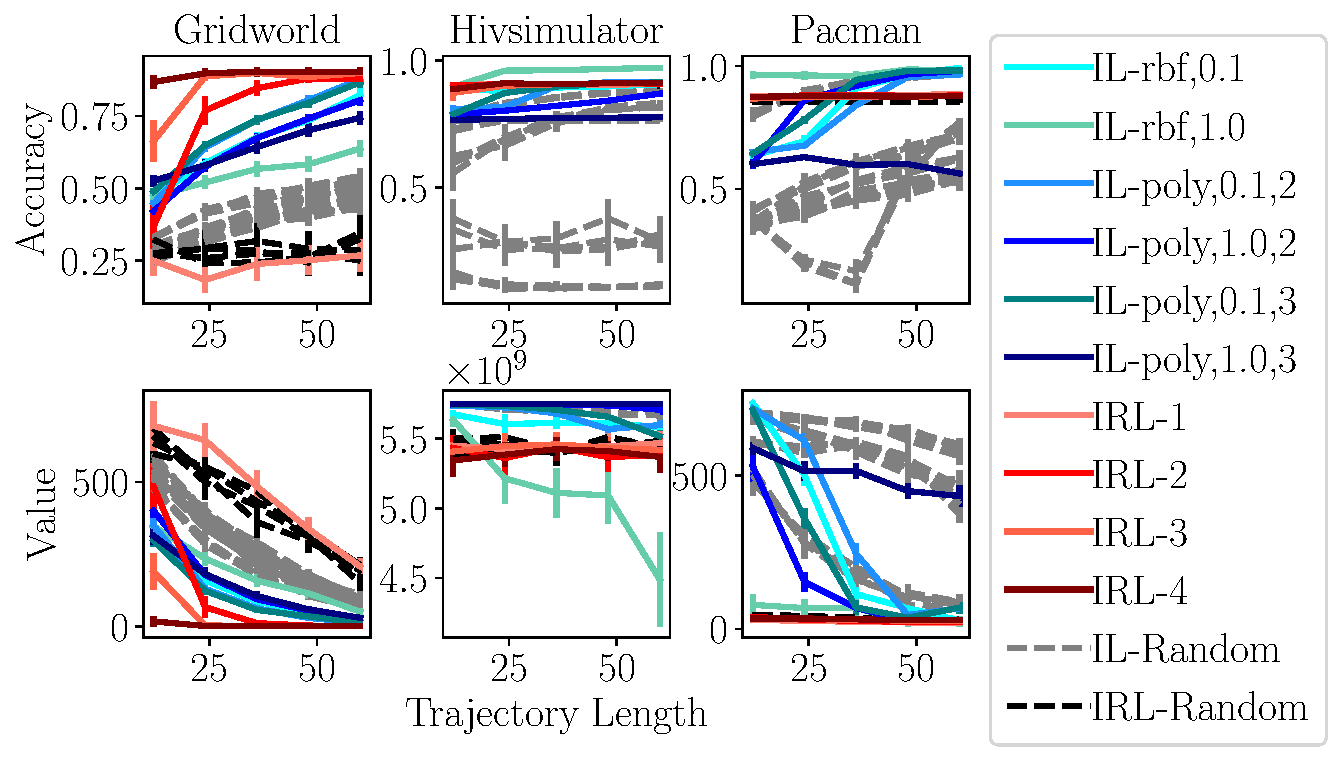
\includegraphics[width=1\columnwidth]{figures/reconstruction_by_summary_size_hyperparams.pdf}
\caption{Reconstruction accuracy across a variety of reconstruction methods and hyper-parameter settings (assuming the same extraction method), by summary size, averaged over 5 random restarts. We include standard error bars but they are generally too small to see. Some methods completely dominate others; we further investigate the robustness of best-performing methods in Figure~\ref{fig:computationalResults}.}
\label{fig:hyperparameters}
\vspace{-0.4cm}
\end{figure}

\begin{figure*}
\centering
\begin{tabular}{ccc}
\subcaptionbox{Random Grid World}{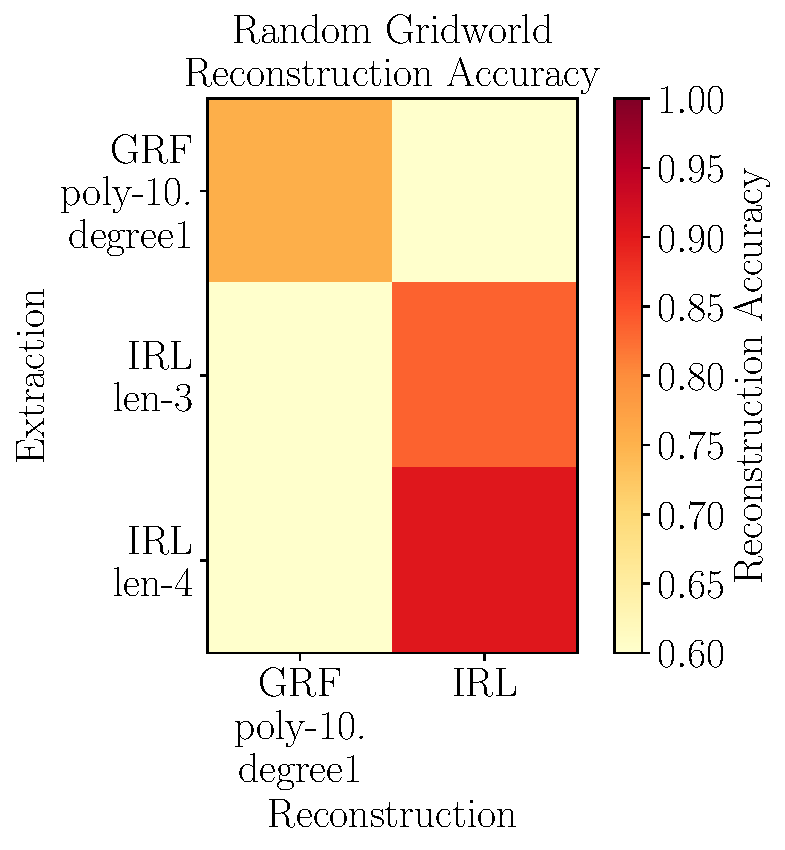
\includegraphics[width=0.25\linewidth]{figures/accuracy_table_randomgridworld.pdf}} &
\subcaptionbox{Pacman}{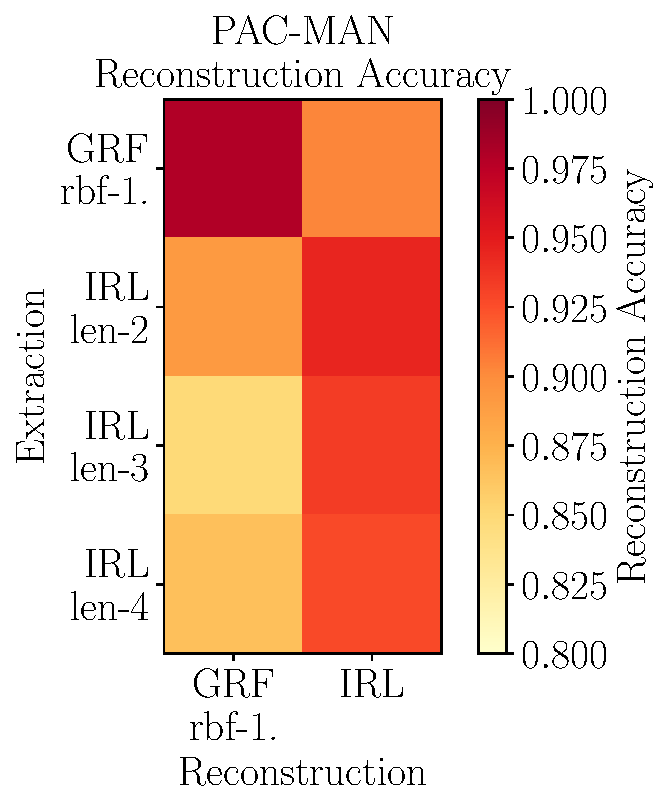
\includegraphics[width=0.25\linewidth]{figures/accuracy_table_pacman.pdf}} &
\subcaptionbox{HIV Simulator}{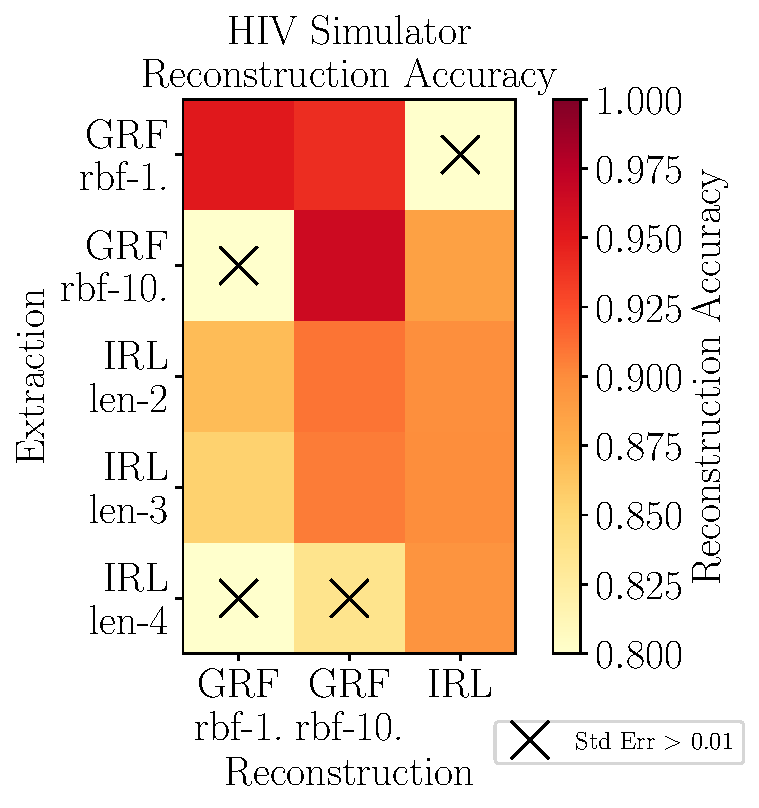
\includegraphics[width=0.25\linewidth]{figures/accuracy_table_hivsimulator.pdf}}
\end{tabular}
\caption{Accuracy averaged over 20 random restarts of every reconstruction model used for summary extraction with summaries extracted with each model. The rows correspond to extraction models and the columns correspond to reconstruction models. The number following the kernel type indicates the length scale. All reconstruction models reconstruct the policy most accurately with the matched summary extraction model. In the PAC-MAN and HIV domains, some summary extraction models are more robust to misspecification of the reconstruction model than others; in the random gridworld domain, no summary extraction models are robust to misspecification.}
\label{fig:computationalResults}
\vspace{-0.2cm}
\end{figure*}

\paragraph{Across all datasets, all models reconstruct the policy most accurately when the summary is extracted using the same model.} In Figure \ref{fig:computationalResults}, the accuracy for each column (corresponding to the reconstruction model) is highest for the row (corresponding to the extraction model), when the reconstruction model and extraction model match. Note that for IRL, there are several summaries extracted with different trajectory lengths that all correspond to the same IRL reconstruction method. This suggest that both the IL and IRL methods extract summaries that allow the model assumed during summary extraction to reconstruct the policy accurately. 

\paragraph{In some cases, using any model of human computation other than the correct one during extraction leads to poor reconstruction.}
In the random gridworld domain, which involves tiles with different rewards, the IRL model reconstructs the policy with higher accuracy than the IL model. This makes sense, as the agent's behavior in this domain was determined using value iteration where the reward function was defined as a linear function of the state features, so IRL had a clear advantage over IL. Despite this, the IL model in Figure~\ref{fig:computationalResults}(a) (top row) can still produce summaries that the model can reconstruct with accuracy of $0.75 \pm 0.002$.

More interestingly, in this domain, the IRL model cannot reconstruct the policy well with this summary, and the IL model cannot reconstruct the model well with the summary extracted with the IRL models. This suggests that in some settings, none of the models we use to extract summaries are robust to a mismatch between the model used during summary extraction and the model used for reconstruction; in such settings we must make sure that we have an accurate model of human computation for the reconstruction.

\paragraph{In other settings, some summaries are more robust to a mismatch between summary extraction and reconstruction models than others.} In PAC-MAN (Figure~\ref{fig:computationalResults}(b)), the summary extracted with IRL and trajectory length 2 (second row) allows the GRF model with length scale 1 (first column) to reconstruct the policy with higher accuracy than the summaries generated with other choices of trajectory length (rows 3 and 4). In the HIV simulator (Figure~\ref{fig:computationalResults}(c)), the summary extracted with the GRF model with RBF kernel and length scale 10 (second row) allows the IRL model to reconstruct the policy more accurately than the GRF model with RBF kernel and length scale 1 (row 1). The summaries extracted with the IRL model with trajectory lengths 2 and 3 (third and fourth rows) allow both GRF models (first and second columns) to reconstruct the policy more accurately than the summary extracted with the IRL model and trajectory length 4 (fifth row). This suggests that under certain settings, there may exist models of human computation that will produce summaries that are robust across a variety of true models, and this property can be checked simply via computation (that is, without user studies). 

Related, we see that hyperparameter choices also affect the robustness of the reconstruction. Specifically, in the HIV domain, we see that one hyperparameter setting of IL model was more robust to misspecified hyperparameters than the other: The summary extracted with the IL model with RBF kernel and gamma 1 (row 1) allows the other IL model (row 2) to reconstruct the summary accurately, while the summary extracted with the IL model with RBF kernel and gamma 10 (row 2) does not. Whether it is important to match both the model class and the hyperparameter settings to human mental models, or whether it is enough to get the model class right is an area for future work. 

[Ike: I want to rethink this part, but I don't know whether to remove it or to do it differently.  Maybe depends on the user study?  For now, I think we can ust cut it!]

\paragraph{A mismatch in features may result in poor reconstruction.} In the PAC-MAN domain, we experimented with giving the agent two different ways to represent its state. As can be seen in Table~\ref{fig:featureMismatch}, if we extract a summary with any of the methods used in figure~\ref{fig:computationalResults}(b), neither the GRF with the features derived for IRL nor the IRL with the features derived for IL is able to reconstruct the policy with any summary with reasonable accuracy. While this is not surprising, it suggests that even if we extract summaries using a model that matches how humans generalize, we may not produce good summaries if we do not also use the same set of features that the human is using to characterize states.

\begin{table}[]
\small
\resizebox{0.9\columnwidth}{!}{
\begin{tabular}{|p{2cm}|p{2.7cm}|p{2.6cm}|}
\hline
\textbf{Extraction Model} & \textbf{Reconstruction Model} & \textbf{Reconstruction Accuracy $\pm$ Std Err}\\
\hline
GRF-rbf, 1.0 & GRF-rbf,1.0-IRL feat. & 0.349 $\pm$ 0.002 \\ 
\hline
GRF-rbf,1.0 & IRL-IL feat. & 0.567 $\pm$ 0.000 \\
\hline
IRL-trajlen2 & GRF-rbf,1.0-IRL feat. & 0.321 $\pm$ 0.002 \\
\hline
IRL-trajlen2 & IRL-IL feat. & 0.567 $\pm$ 0.000 \\
\hline
IRL-trajlen3 & GRF-rbf,1.0-IRL feat. & 0.333 $\pm$ 0.003 \\
\hline
IRL-trajlen3 & IRL-IL feat. & 0.553 $\pm$ 0.000 \\
\hline
IRL-trajlen4 & GRF-rbf,1.0-IRL feat. & 0.353 $\pm$ 0.002 \\
\hline
IRL-trajlen4 & IRL-IL feat. & 0.581 $\pm$ 0.001 \\
\hline
\end{tabular}}
\caption{For each summary in Figure~\ref{fig:computationalResults}(b), we compute the reconstruction accuracy with every model with features derived for the other model (i.e. we use the features derived for IRL to do IL and vice versa). No reconstruction model achieves accuracy higher than 0.6.}
\label{fig:featureMismatch}
\vspace{-0.9cm}
\end{table}

\section{Human-Subject Study}
Our computational experiments showed that a mismatch between summary extraction methods and the methods used to reconstruct a policy can lead to wrong generalizations. We conducted a preliminary user study to assess people's reconstruction strategies, and in particular, their ability to extrapolate from summaries optimized for IL or IRL reconstruction methods.

\subsection{Empirical Methodology}
\paragraph{Participants} 71 participants were recruited through Amazon Mechanical Turk (28 female, Mean age = 39.69, STD = 12.27). 
Participants received a base payment of \$1.5, and could earn a bonus of up to \$1 with respect to the percentage of correct answers.

\paragraph{Task} In the experiment, participants were shown summaries of agents using different policies to navigate 2-D maps. The maps consist of colored tiles on a 2-D grid, where colors correspond to state features. The summary shows how the agent acts in some parts of the map by displaying arrows corresponding to actions in some tiles. Each summary was generated to allow accurate reconstruction of the policy with either IRL or IL. Because the IRL-based approach extracts trajectories of states, in those summaries we used arrows of different colors to indicate separate agent trajectories. 

Participants were asked to predict which action the agent would take in states shown on a different 2-D grid, if it employs the same strategy presented in the summary. These states were shown next to the summary, such that participants could inspect the summary while making their predictions. Figure~\ref{fig:interface} shows example action prediction tasks for IRL-based and IL-based summaries. Participants were also asked to report their confidence in their prediction on a 7-point Likert scale (1 - not at all confident to 7 - very confident).

\begin{figure*}
\centering
\begin{tabular}{cc}
\subcaptionbox{Inverse Reinforcement Learning}{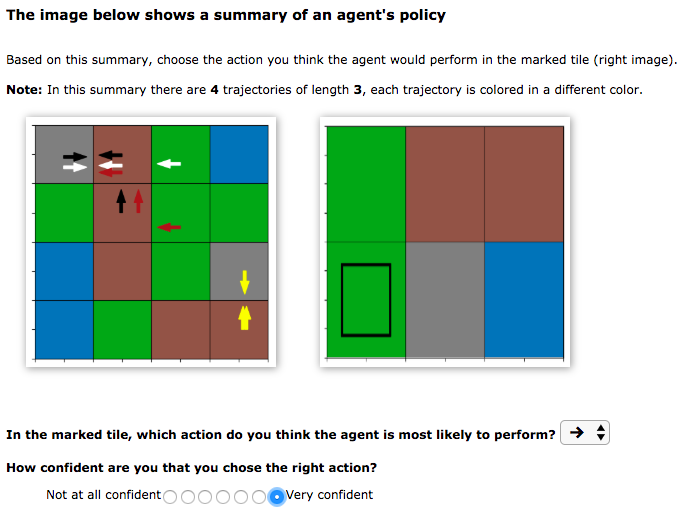
\includegraphics[width=0.4\linewidth]{figures/interface_irl.png}} &
\subcaptionbox{Imitation Learning}{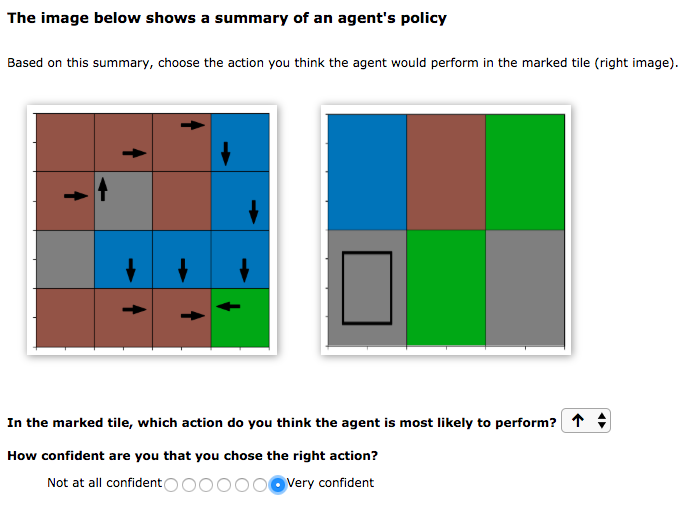
\includegraphics[width=0.4\linewidth]{figures/interface_il.png}} \\
\end{tabular}
\caption{Experimental interface. (a) an IRL-based summary and action prediction task; (b) and IL-based summary and action prediction task. Arrows indicate the agent's actions in different states in the grid; the IRL approach extracts summaries that visit the same state multiple times--denoted with offset arrows, while the IL approach does not. Participants are asked to predict the action for tiles (shown in a square) on a different grid.}
\label{fig:interface}
\vspace{-0.2cm}
\end{figure*}

The summaries were displayed on a 4x4 grid, with 4 binary features per cell representing different colors. The test grids used for the prediction task were of size 2x3 and were created for each policy and summary method. In all grids, states correspond to the grid cells, where for each state only one of the binary features was active. The possible actions were moving in four directions (up, down, left and right), where the agent could not take actions causing it to leave the grid borders. For each policy, We created two state-feature mappings: one for IL, mapping state features to actions, and the other for IRL, mapping state features to rewards.

We used a summary budget of 12, i.e., each summary showed 12 state-action pairs. IRL-based summaries were extracted using machine teaching, with trajectories of length 3 (for a total of 4 trajectories). Summaries were extracted for IL by choosing a state of each color and then filling with random states to get a summary of the same size; in this small domain, active learning was not needed. We use an SVM with a linear kernel to measure reconstruction since this was sufficient to capture this simple policy.

The feature representation of states, test grids and the policies to be summarized were handcrafted such that each summary obtained reconstruction accuracy of 1.0 if the extraction model matched the reconstruction model, and obtained an accuracy of less than 0.5 if the extraction model did not match the reconstruction model. (Reconstruction accuracy was computed for the policy states not shown in the summary, and for all states in the test grid.) We chose this setup to see whether participants would employ the correct reconstruction method, or whether they would use the same reconstruction methods for different summaries, which we expect to result in low accuracy.

\paragraph{Procedure} Participants were first shown a tutorial explaining the grid world properties and the structure of the summaries. To avoid biasing participants toward a particular reconstruction method, they were only told that the agent's behavior is in some way related to the colors of tiles, but they were not told whether colors map to actions (IL) or to rewards (IRL). Then, they had to pass a quiz ensuring they read and understood the instructions. Next, they were asked to complete the task described above for summaries of four different agent policies, two extracted using IRL and two using IL. For each summary, after making all predictions, participants were asked to provide a brief text description of the agent's behavior.

The first two tasks were considered training tasks (though this was not mentioned to the participants), intended to familiarize them with the domain and interface. In the training phase, participants were shown one IRL and one IL summary, and asked to predict the action only in two tiles of the test grid. Next, they were shown two more summaries, one IRL and one IL, and were asked to predict the action taken by the agent in each of the tiles in the test grid (6 in total). The order in which the  IRL and IL summaries were shown was randomized to avoid bias due to learning effects. The assignment of summary extraction method to agent policies was also randomized to avoid potential effects of different generalization difficulty levels for different policies. For each grid, participants were asked to predict actions for each empty tile one at a time. We used a within-subject study design, such that all participants evaluated both summary methods. 
%Ike: is this what we did? Do we need more details? Ofra: I think this is fine (I added that the assignment of summary method to policy was also randomized)

\subsection{Results}
As shown in Figure~\ref{fig:user_study_results}(a), participants were able to predict the agent's actions much more accurately when given summaries extracted by the IL method than for those extracted with IRL (Mean correct answers: IL = 0.89, IRL = 0.39). Moreover, participants took twice as long to predict each action when shown the IRL-based summaries compared to IL-based summaries (Mean time in seconds: IL = 8.96, IRL = 16.16), see figure \ref{fig:user_study_results}(b). The differences in accuracy and time were statistically significant ($p<0.001$ in both cases, using Wilcoxon signed-ranked test).
We conducted another study on a small group of participants ($N=18$) where we showed only summaries extracted using IRL, to test whether participants are fixated by the IL summaries (although IL and IRL summaries were shown in an alternating order). The mean percent of correct answers increased from 0.39 to 0.6, but remained significantly lower than for the IL summaries (0.89). 

Looking at the explanations provided for each summary, we observed that for the IL summaries most participants based their predictions on a mapping of colors to actions, naturally using IL for reconstruction. E.g. ``Blue moves left, grey moves down, brown moves right, green moves up" or "Direction was based on color''. This behavior implies that participants were imitating the agent behavior they observed in the summary. For the IRL summaries, the explanations indicate that participants had difficulty understanding the agent behavior. Many of them still tried mimicking the actions presented in the summary, e.g ``he was all over the place but I tried to mimic the direction on the color''. Some participants also based their explanations on directional behavior regardless of color, e.g. ``The agent seemed to always go down if it could''. This emphasizes the effect of prior assumptions people make regarding a domain on their comprehension---even though participants were explicitly told (and answered a quiz question) that the behavior was only affected in some way by colors, some of them still assumed the agent was trying to get to a certain location or move in a certain pattern. There were only few participants that noticed the different colors have different values to the agent, and that the actions are taken accordingly to obtain the highest value, e.g. ``Preference of color (move cost). High to low: green, blue, brown, grey''. 

Confidence ratings for IL summaries were higher when participants were correct in their predictions, compared to when they were wrong (mean confidence: correct = 5.72, incorrect = 5.0,$p = 0.0003$). As opposed to that, for the IRL summaries the differences in confidence between correct and incorrect answers was insignificant (mean confidence: correct = 4.16, incorrect = 4.01, $p = 0.26$). Also, the mean confidence for IRL summaries was significantly lower than reported for IL (IRL = 4.07, IL = 5.65, $p<0.001$). These results are in line with the descriptive explanations provided by the participants, showing they were more confident in their predictions based on IL summaries. 

\begin{figure}
\centering
\begin{tabular}{cc}
\subcaptionbox{}{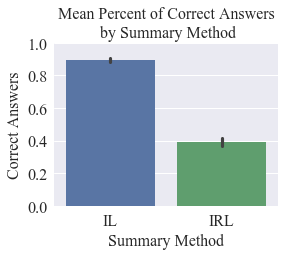
\includegraphics[width=0.45\columnwidth]{figures/user_study_correct_rate.png}} &
\subcaptionbox{}{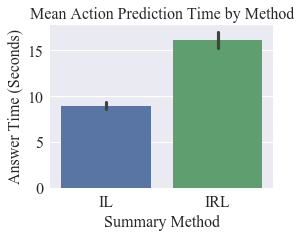
\includegraphics[width=0.45\columnwidth]{figures/user_study_time.png}}
\end{tabular}
\caption{Participants were more accurate when predicting actions, and responded faster, when shown IL-based summaries. (a) Mean accuracy of participants using IRL-based and IL-based summaries; (b) Mean response times for action prediction when shown IRL-based and IL-based summaries.}
\label{fig:user_study_results}
\vspace{-0.4cm}
\end{figure}

\section{Discussion \& Future Work} 
Summaries of agent policies have potential to improve human users' understanding of agents' behavior. In this paper, we investigated different approaches for extracting policy summaries, which differ in their assumptions about the methods that might be used by people to extrapolate from these summaries and reconstruct an agent's policy. We conducted computational experiments to investigate the effect of using different computational models both for summary extraction and for policy reconstruction. 

Specifically, we explored, both computationally and through user studies, differences between summaries that presume that the human will use a future-value oriented way of processing a summary (IRL) or use a mimic-based approach (IL). Across different types of domains, we found that different models of computation might be preferred. We also found that for any given reconstruction model used, the highest policy reconstruction accuracy was achieved when the summary was extracted using the same model. While in some domains there were summaries that were fairly robust to different reconstruction models, in other domains it was crucial that the extraction and reconstruction models match. Moreover, we found that matching between the feature representation used for summary extraction and policy reconstruction can also be important, with mismatch resulting in low reconstruction accuracy.

While we explored several variants of each IL and IRL, there are many design choices. For example, we defined the optimization goal as predicting the agent's behavior in unseen states; prior work has considered accurately modeling the reward function~\cite{huang17communicate}, or including ``important'' states, as measured by Q-value differences~\cite{amir2018highlights, huang2018establishing}. For the optimization procedures, our machine teaching approach for IRL stopped at a fixed budget, even if perfect recovery was not achieved; our active learning for IL was chosen because it was computationally-efficient (methods with guarantees do exist, e.g. \cite{liu2016teaching}, but do not account for sets of fixed size, or the requirement to only include examples that exist in a dataset). Finally, we used a Gaussian random field model for IL and the Max-Ent approach for IRL; we could have chosen other classifiers and IRL approaches.

%Ike: I think this is the paragraph above? [ADD: NOTE about reasons our summaries/reconstructions may not have been perfect] 

That said, with the variation we capture, our results emphasize the importance of selecting summaries that align with users' policy reconstruction model and feature representation. The results are further supported through a preliminary human-subject study, which showed that people failed to predict an agent's policy when their reconstruction strategy did not match the strategy for which summaries were optimized. In our experiment, people tended to make imitation learning-based inferences, causing them to fail to extrapolate from summaries optimized for reconstruction with IRL. 
%Through computational experiments, we showed that different summary extraction methods might result in higher reconstruction accuracy depending on the domain, and that a mismatch between extraction and reconstruction methods can result in a failure to reconstruct an agent's policy. 

%Our empirical results emphasize the importance of selecting summaries that align with users' policy reconstruction. 

Predicting which reconstruction strategies people will deploy can be difficult, since their strategies can vary depending on the context and their a priori knowledge and assumptions about the domain and the agent's behavior; importantly, different users might deploy different reconstruction strategies. In cases where some extraction model is robust across different reconstruction models, summaries based on the model might be beneficial even if people use different reconstruction approaches. However, since our results show that in some domains there might not be a robust extraction model, and that feature representation alignment between extraction and reconstruction also substantially impacts the ability to recover a policy, finding robust summaries might not be feasible.

To address this problem, one approach for future work could be a human-in-the-loop summary extraction process that first elicits users' reconstruction method and feature representation and then extracts summaries that align with the user's model. Another option would be to use user-studies to identify in which types of situations people generally choose one reconstruction approach over the other, as well as learn ways to prime users to use the reconstruction approach which could result in better generalization for a given domain. Given the variability that we see in reconstruction across different types of domains, these kinds of studies will be essential for endowing users with accurate mental models of agents; our work demonstrates that simply showing trajectories, even intelligently chosen to be robust, will not be sufficient.


\small
\bibliographystyle{named}
\bibliography{bibliography}

\end{document}
